\documentclass[a4paper,oneside,11pt]{book}

\usepackage[utf8]{inputenc}
\usepackage[spanish,activeacute]{babel}
%\usepackage[T1]{fontenc}
\usepackage{tabulary}
\usepackage{graphicx}
\usepackage{float}

\oddsidemargin=0.2cm
\headsep=1cm
\textheight=21cm
\textwidth=16cm

\begin{document}
% cuerpo del documento
\title{Metodología de Desarrollo Software}
\author{Pablo Eduardo Ojeda Vasco}
\date{\today}

\maketitle

% section  (end)
%%%%%%%%%%%%%%%%%%%%%%%%%%%%%%%%%%%%%%
% Entrega 1. Lista de características
%%%%%%%%%%%%%%%%%%%%%%%%%%%%%%%%%%%%%%
\chapter{Lista de características}
% 1.1.- Introducción
\section{Introducción}
% 1.1.1.- Descripción general del proyecto
\subsection{Descripción general del proyecto}
El {\bf dominio} de la aplicación es el de las {\bf consultas médicas privadas}, donde normalmente existen {\bf dos actores} principales: el médico y el paciente. Es decir, el proyecto está orientado a médicos que gestionen consultas de carácter particular y a sus pacientes.

	En primer lugar debemos ponernos en situación. En el sector de la sanidad privada, la gestión de centros médicos (desde el seguimiento de un paciente hasta la organización interna del mismo) se ha desarrollado {\bf tradicionalmente en papel} (información analógica). Sin embargo, con el avance tecnológico y con la aparición de las nuevas tecnologías de información y comunicación (TICs), se crean nuevos modelos de gestión y administración de los centros, pasando todos los flujos de datos a versión digital. Es decir, la información comienza a gestionarse usando software específico, pero {\bf centralizado en una localización física concreta}. A pesar de todo, sigue habiendo muchos especialistas que no han dado el paso y continúan utilizando métodos arcaicos.

	Por otro lado, {\bf el proceso de concertar una cita} sigue siendo el mismo que antaño: un paciente debe presentarse en la consulta del médico físicamente y solicitar cita ó bien debe realizar una llamada telefónica para ser atendido por un administrativo.

	Por tanto, con el objetivo de poder gestionar digitalmente y desde “la nube” todos los aspectos referentes al flujo de información de una consulta médica, se requiere desarrollar una aplicación web desde la que se gestionen un gran número de consultas privadas, con todos los datos referentes a médicos (curriculum, precios, horarios de disponibilidad, etc.), a pacientes (ficha médica, diagnósticos, pruebas, exploraciones, etc.), los pagos y el seguimiento de la contabilidad y además, permita que sean los propios especialistas los que muestren a los pacientes de que horas libres disponen, para que sean estos últimos los encargados de asignarse, desde cualquier ubicación en la que exista un computador con internet, la cita que más les convenga.

% 1.1.2.- Usuarios
\subsection {Usuarios}
He realizado una clasificación de los posibles usuarios del sistema. De esta forma podremos identificar y asociar cada característica con cada uno de ellos. 
	
\begin{itemize}
\item \textbf{Médicos.} A ellos está dedicada la aplicación. Pueden tener cualquier tipo de especialidad.
\item \textbf{Pacientes.} No son los usuarios principales del sistema, pero son el sustento de los médicos. Pueden interactuar con el software a la hora de reservar citas o de realizar pagos por adelantado.
\item \textbf{Administrador del sistema.} Encargado de verificar que el sistema funciona correctamente. Además, debe verificar que un médico esté licenciado como tal y realizar las copias de seguridad.
\end{itemize}

% 1.2.- Objetivos
\section{Objetivos}
Se propone diseñar e implementar una aplicación SaaS (Software as a Service), que lo que pretende es ofertar un {\bf software como servicio} a todos aquellos especialistas sanitarios interesados. 

	Por tanto, se desarrollará una aplicación web, en la que se abordaran los siguientes módulos:
\begin{itemize}
\item \textbf{Gestión de pacientes.} Ficha médica de los pacientes, con sus pruebas médicas, diagnósticos e información asociada.
\item \textbf{Gestión de médicos.} Información acerca de los especialistas.
\item \textbf{Gestión de administrador.} Para un administrador del sistema, encargado de las copias de seguridad, debido a que al estar centrado en sanidad, tiene un nivel de protección de datos de alta prioridad.
\item \textbf{Gestión de horarios de los pacientes.} Permite a los pacientes buscar y gestionar sus citas.
\item \textbf{Gestión de horario de disponibilidad del médico.} Permite a los especialistas establecer su horario de disponibilidad.
\item \textbf{Módulo de Gestión de pagos.} Para poder realizar pagos vía paypal.
\item \textbf{Módulo de Gestión de contabilidad.} Controla los ingresos y gastos en los centros.
\end{itemize}

% 1.3.- Lista de características
\section{Lista de características}
La lista de características es un artefacto que se obtiene después de aplicar la tarea de “Enumerar los requisitos candidatos”, que se propone en la metodología del PUD (Proceso Unificado de Desarrollo), para la captura de requisitos. 
	
	Esta lista contiene las ideas de clientes, usuarios, analistas y desarrolladores sobre posibles aspectos que se podrían incluir en la aplicación, y que, posteriormente, se podrán traducir en requisitos del software. 

	Estas ideas se consideran requisitos candidatos que se podrán desarrollar en la versión actual del sistema o se podrán postergar a versiones futuras. Este artefacto sirve para gestionar el proyecto y sólo se utiliza para la planificación del trabajo. Podrá ir variando a medida que avance el proyecto, pudiéndose añadir y modificar las características que se crean oportunas, en cualquier momento del desarrollo.

% 1.3.1.- Descripción de las características
\subsection{Descripción de las características}
Para describir cada una de las características vamos a utilizar los siguientes campos:

\begin{itemize}
\item \textbf{Código.} Identifica a la característica. Se especifica como Categoría + Número. Las categorías se especifican más abajo.
\item \textbf{Nombre.} El nombre de la característica.
\item \textbf{Descripción.} Breve descripción de lo que comprende la característica.
\item \textbf{Estado.} Cada característica tendrá un estado que irá variando a medida que progrese el proyecto. Los posibles estados son:
	\begin{itemize}
		\item Aceptado. Se desarrollará en esta versión del producto.
		\item Rechazado. No se desarrollará.
		\item Postergado. Se desarrollará en una futura versión.
		\item En desarrollo. Ya se está desarrollando.
		\item Finalizado. Se ha concluido.
	\end{itemize}
\item \textbf{Prioridad.} Determinará el orden en el que se van a ir desarrollando. Los tipos de prioridades son:
	\begin{itemize}
		\item Muy alta.
		\item Alta.
		\item Media.
		\item Baja.
		\item Muy Baja.
	\end{itemize}
\item \textbf{Riesgo.} Representa la dificultad para conseguir implementar la característica correctamente. Existen tres niveles: 
	\begin{itemize}
		\item Crítico
		\item Significativo
		\item Rutinario.
	\end{itemize}
\end{itemize}

% 1.3.2.- Categorías
\subsection{Categorías}
Para organizar la lista tenemos una serie de categorías que se mencionan a continuación. Gracias a esto podremos gestionar mejor la lista de características.
\begin{itemize}
\item [A].- Gestión de Actividades Generales 
\item [B].- Gestión de información de médicos.
\item [C].- Actividades de los médicos.
\item [D].- Gestión de pacientes.
\item [E].- Gestión de fichas médicas de pacientes.
\item [F].- Gestión de horarios de los médicos.
\item [G].- Gestión de citas de los pacientes.
\item [H].- Consulta y Diagnósticos.
\item [I].- Gestión de cobros y pagos.
\item [J].- Gestión de contabilidad.
\item [K].- Panel de Administrador.
\item [L].- Otros
\end{itemize}

% 1.3.3.- Lista de características
\subsection{Lista de características}

%%%%%%%
% A - Gestión de actividades generales
%%%%%%%
\subsubsection{A.- Gestión de actividades generales.}

%\begin{table}
\begin{center}
\begin{tabulary}{15cm}{|L|}
	\hline
		\bf{A.1.- Tour de la Aplicación} \\
	\hline
		Cualquier médico ó paciente podrá hacer una visita guiada sobre las principales funcionalidades de la aplicación.\\
	\hline
		Prioridad \textit{Medio.} \\
	\hline
		Estado \textit{Postergado.} \\
	\hline
		Riesgo \textit{Riguroso.} \\
	\hline
\end{tabulary}
\end{center}
%\caption{XXX}
%\end{table}

%\begin{table}
\begin{center}
\begin{tabulary}{15cm}{|L|}
	\hline
		\bf{A.2.- Registrarse como médico} \\
	\hline
		Un médico deberá registrarse como tal. Se pasará a rellenar una serie de datos correspondientes con su información personal, profesional, etc. El usuario será el e-mail seleccionado, y su contraseña la elegida.\\
	\hline
		Prioridad \textit{Muy Alta.} \\
	\hline
		Estado \textit{Aceptado.} \\
	\hline
		Riesgo \textit{Significativo.} \\
	\hline
\end{tabulary}
\end{center}
%\caption{XXX}
%\end{table}

%\begin{table}
\begin{center}
\begin{tabulary}{15cm}{|L|}
	\hline
		\bf{A.3.- Registrarse como paciente.} \\
	\hline
		Un paciente deberá registrarse como tal. Se pasará a rellenar una serie de datos correspondientes con su información personal, sus historial médico, etc. El usuario será el e-mail seleccionado y su contraseña la elegida. \\
	\hline
		Prioridad \textit{Muy Alta.} \\
	\hline
		Estado \textit{Aceptado.} \\
	\hline
		Riesgo \textit{Significativo.} \\
	\hline
\end{tabulary}
\end{center}
%\caption{XXX}
%\end{table}

%\begin{table}
\begin{center}
\begin{tabulary}{15cm}{|L|}
	\hline
		\bf{A.4.- Registrarse como administrativo.} \\
	\hline
		Un administrativo deberá registrarse como tal. El usuario será el e-mail seleccionado y su contraseña la elegida. Deberá permanecer a la espera de que su médico le autorice. \\
	\hline
		Prioridad \textit{Baja.} \\
	\hline
		Estado \textit{Rechazado.} \\
	\hline
		Riesgo \textit{Significativo.} \\
	\hline
\end{tabulary}
\end{center}
%\caption{XXX}
%\end{table}

%\begin{table}
\begin{center}
\begin{tabulary}{15cm}{|L|}
	\hline
		\bf{A.5.- Rellenar información personal.} \\
	\hline
		Tanto médicos como pacientes debe rellenar todos sus datos personales cuando ingresen en el sistema. Nombre, apellidos, DNI, teléfono de contacto, e-mail, etc. \\
	\hline
		Prioridad \textit{Alta.} \\
	\hline
		Estado \textit{Aceptado.} \\
	\hline
		Riesgo \textit{Riguroso.} \\
	\hline
\end{tabulary}
\end{center}
%\caption{XXX}
%\end{table}

%\begin{table}
\begin{center}
\begin{tabulary}{15cm}{|L|}
	\hline
		\bf{A.6.- Modificar información personal.} \\	
	\hline
		Tanto médicos como pacientes debe poder cambiar algunos de sus datos personales en cualquier momento que desee. \\
	\hline
		Prioridad \textit{Media.} \\
	\hline
		Estado \textit{Aceptado.} \\
	\hline
		Riesgo \textit{Riguroso.} \\
	\hline
\end{tabulary}
\end{center}
%\caption{XXX}
%\end{table}

%\begin{table}
\begin{center}
\begin{tabulary}{15cm}{|L|}
	\hline
		\bf{A.7.- Adjuntar foto del perfil.} \\
	\hline
		Es recomendable que todos los médicos y pacientes tengan una foto del perfil. Respecto a los médicos da mayor seguridad y credibilidad a sus futuros pacientes potenciales. Respecto a los pacientes, permite que los médicos puedan poner cara a la hora de ver los datos. \\
	\hline
		Prioridad \textit{Media.} \\
	\hline
		Estado \textit{Aceptado.} \\
	\hline
		Riesgo \textit{Riguroso.} \\
	\hline
\end{tabulary}
\end{center}
%\caption{XXX}
%\end{table}

%\begin{table}
\begin{center}
\begin{tabulary}{15cm}{|L|}
	\hline
		\bf{A.8.- Modificar foto del perfil.} \\
	\hline
		Tanto médicos como pacientes pueden modificar la foto de su perfil en cualquier momento que desee. Para modificarla deben primero haberla adjuntado. \\
	\hline
		Prioridad \textit{Baja.} \\
	\hline
		Estado \textit{Aceptado.} \\
	\hline
		Riesgo \textit{Riguroso.} \\
	\hline
\end{tabulary}
\end{center}
%\caption{XXX}
%\end{table}

%\begin{table}
\begin{center}
\begin{tabulary}{15cm}{|L|}
	\hline
		\bf{A.9.- Acceso y Autentificación.} \\
	\hline
		Una vez registrado en el sistema, tanto médico, pacientes como administrador deben autentificarse mediante su usuario y contraseña para poder acceder a la aplicación. \\
	\hline
		Prioridad \textit{Muy Alta.} \\
	\hline
		Estado \textit{Aceptado.} \\
	\hline
		Riesgo \textit{Crítico.} \\
	\hline
\end{tabulary}
\end{center}
%\caption{XXX}
%\end{table}

%\begin{table}
\begin{center}
\begin{tabulary}{15cm}{|L|}
	\hline
		\bf{A.10.- Conectarse desde cuenta Facebook.} \\
	\hline
		Un usuario también podrá acceder con su usuario y contraseña de acceso a Facebook. Esto no quita que deba seguir rellenando su información personal y otra serie de datos. \\
	\hline
		Prioridad \textit{Baja.} \\
	\hline
		Estado \textit{Rechazado.} \\
	\hline
		Riesgo \textit{Riguroso.} \\
	\hline
\end{tabulary}
\end{center}
%\caption{XXX}
%\end{table}

%\begin{table}
\begin{center}
\begin{tabulary}{15cm}{|L|}
	\hline
		\bf{A.11.- Recordar contraseña.} \\
	\hline
		Se establece la opción de que el propio navegador recuerde el usuario y la contraseña para que se acceda directamente al sistema sin tener que estar continuamente introduciendo dicha información. \\
	\hline
		Prioridad \textit{Media.} \\
	\hline
		Estado \textit{Aceptado.} \\
	\hline
		Riesgo \textit{Significativo.} \\
	\hline
\end{tabulary}
\end{center}
%\caption{XXX}
%\end{table}

%\begin{table}
\begin{center}
\begin{tabulary}{15cm}{|L|}
	\hline
		\bf{A.12.- Cambiar contraseña.} \\
	\hline
		En cualquier momento que desee, tanto médicos, pacientes como el administrador del sistema podrán cambiar su contraseña de acceso al sistema. Se pedirá contraseña actual para corroborar que es la persona que dice ser y la nueva contraseña deberá introducirse dos veces para evitar errores al teclear. \\
	\hline
		Prioridad \textit{Media.} \\
	\hline
		Estado \textit{Aceptado.} \\
	\hline
		Riesgo \textit{Riguroso.} \\
	\hline
\end{tabulary}
\end{center}
%\caption{XXX}
%\end{table}

%\begin{table}
\begin{center}
\begin{tabulary}{15cm}{|L|}
	\hline
		\bf{A.13.- Cambiar idioma.} \\
	\hline
		Un usuario del sistema, tanto médico, paciente o administrador, podrá cambiar el idioma de la aplicación. \\
	\hline
		Prioridad \textit{Baja.} \\
	\hline
		Estado \textit{Postergado.} \\
	\hline
		Riesgo \textit{Crítico.} \\
	\hline
\end{tabulary}
\end{center}
%\caption{XXX}
%\end{table}

%\begin{table}
\begin{center}
\begin{tabulary}{15cm}{|L|}
	\hline
		\bf{A.14.- Contactar con el Administrador.} \\
	\hline
		En caso de cualquier consulta o problema, los médicos podrán enviar directamente un email al administrador. \\
	\hline
		Prioridad \textit{Baja.} \\
	\hline
		Estado \textit{Aceptado.} \\
	\hline
		Riesgo \textit{Riguroso.} \\
	\hline
\end{tabulary}
\end{center}
%\caption{XXX}
%\end{table}

%\begin{table}
\begin{center}
\begin{tabulary}{15cm}{|L|}
	\hline
		\bf{A.15.- Términos Legales.} \\
	\hline
		Se expondrán todos los términos legales accesibles para todo el mundo, tanto registrado en el sistema como ajeno a éste. \\
	\hline
		Prioridad \textit{Media.} \\
	\hline
		Estado \textit{Aceptado.} \\
	\hline
		Riesgo \textit{Riguroso.} \\
	\hline
\end{tabulary}
\end{center}
%\caption{XXX}
%\end{table}

%\begin{table}
\begin{center}
\begin{tabulary}{15cm}{|L|}
	\hline
		\bf{A.16.- Condiciones de uso.} \\
	\hline
		Una lista de características con las condiciones de uso del sistema con las que se informará a sus usuarios de todo tipo de detalles respecto a cualquier detalle relacionado con su utilización. \\
	\hline
		Prioridad \textit{Media.} \\
	\hline
		Estado \textit{Aceptado.} \\
	\hline
		Riesgo \textit{Riguroso.} \\
	\hline
\end{tabulary}
\end{center}
%\caption{XXX}
%\end{table}

%\begin{table}
\begin{center}
\begin{tabulary}{15cm}{|L|}
	\hline
		\bf{A.17.- Autocompletar las búsquedas.} \\
	\hline
		Cualquier búsqueda que se realice en el sistema, bien por parte del paciente, del médico o del administrador, se realizará mediante el autocompletado, de forma que se aconseje al usuario sobre las posibles búsquedas posibles. \\
	\hline
		Prioridad \textit{Baja.} \\
	\hline
		Estado \textit{Postergado.} \\
	\hline
		Riesgo \textit{Crítico.} \\
	\hline
\end{tabulary}
\end{center}
%\caption{XXX}
%\end{table}

%\begin{table}
\begin{center}
\begin{tabulary}{15cm}{|L|}
	\hline
		\bf{A.18.- Preguntas frecuentes.} \\
	\hline
		Es siempre muy útil ver un apartado de preguntas y respuestas con las cuestiones más usuales que se pueden plantear los usuarios de la aplicación. \\
	\hline
		Prioridad \textit{Baja.} \\
	\hline
		Estado \textit{Aceptado.} \\
	\hline
		Riesgo \textit{Crítico.} \\
	\hline
\end{tabulary}
\end{center}
%\caption{XXX}
%\end{table}

%\begin{table}
\begin{center}
\begin{tabulary}{15cm}{|L|}
	\hline
		\bf{A.19.- Enlaces a sitios médicos de interés.} \\
	\hline
		Puede resultar atractivo contar con publicidad sobre sitios en los que se hable de medicina y salud. Todo ello sin ánimo de lucro. \\
	\hline
		Prioridad \textit{Baja.} \\
	\hline
		Estado \textit{Rechazado.} \\
	\hline
		Riesgo \textit{Crítico.} \\
	\hline
\end{tabulary}
\end{center}
%\caption{XXX}
%\end{table}

%\begin{table}
\begin{center}
\begin{tabulary}{15cm}{|L|}
	\hline
		\bf{A.20.- Ayuda.} \\
	\hline
		En cualquier momento, cualquier usuario podrá solicitar ayuda sobre cualquier funcionalidad. Además, en cada icono del interfaz gráfica aparecerá al pasar el ratón por encima cuál es su uso. \\
	\hline
		Prioridad \textit{Baja.} \\
	\hline
		Estado \textit{Aceptado.} \\
	\hline
		Riesgo \textit{Crítico.} \\
	\hline
\end{tabulary}
\end{center}
%\caption{XXX}
%\end{table}


%%%%%%%%%%
% B - Gestión de información de médicos
%%%%%%%%%%
\subsubsection{B.- Gestión de información de médicos.}

%\begin{table}
\begin{center}
\begin{tabulary}{15cm}{|L|}
	\hline
		\bf{B.1.- Rellenar número de colegiado.} \\
	\hline
		Cualquier médico debe tener asociado un número de colegiado en el Colegio de Médicos. Dicho identificador debe ser añadido \\
	\hline
		Prioridad \textit{Muy Alta.} \\
	\hline
		Estado \textit{Aceptado.} \\
	\hline
		Riesgo \textit{Riguroso.} \\
	\hline
\end{tabulary}
\end{center}
%\caption{XXX}
%\end{table}

%\begin{table}
\begin{center}
\begin{tabulary}{15cm}{|L|}
	\hline
		\bf{B.2.- Rellenar información del centro (localización, contacto).} \\
	\hline
		Es necesario que un paciente conozca la ubicación de la consulta del médico. Así mismo, debe tener unos datos de contacto, un CIF, etc. \\
	\hline
		Prioridad \textit{Alta.} \\
	\hline
		Estado \textit{Aceptado.} \\
	\hline
		Riesgo \textit{Riguroso.} \\
	\hline
\end{tabulary}
\end{center}
%\caption{XXX}
%\end{table}

%\begin{table}
\begin{center}
\begin{tabulary}{15cm}{|L|}
	\hline
		\bf{B.3.- Adjuntar curriculum.} \\
	\hline
		Se oferta la posibilidad de que un médico adjunte su curriculum en caso de que disponga de este en formato digital. \\ 
	\hline
		Prioridad \textit{Media.} \\
	\hline
		Estado \textit{Aceptado.} \\
	\hline
		Riesgo \textit{Riguroso.} \\
	\hline
\end{tabulary}
\end{center}
%\caption{XXX}
%\end{table}

%\begin{table}
\begin{center}
\begin{tabulary}{15cm}{|L|}
	\hline
		\bf{B.4.- Crear curriculum.} \\
	\hline
		En el caso de no tener un curriculum en formato digital, o de no poder escanear uno, se ofrece la posibilidad de crear su propio curriculum. \\
	\hline
		Prioridad \textit{Baja.} \\
	\hline
		Estado \textit{Postergado.} \\
	\hline
		Riesgo \textit{Significativo.} \\
	\hline
\end{tabulary}
\end{center}
%\caption{XXX}
%\end{table}


%%%%%%%%%%
% C - Actividades de los médicos
%%%%%%%%%%
\subsubsection{C.- Actividades de los médicos.}

%\begin{table}
\begin{center}
\begin{tabulary}{15cm}{|L|}
	\hline
		\bf{C.1.- Enviar certificación de licencia médica.} \\
	\hline
		Para poder corroborar que un médico tiene licencia médica, éste debe mandar una copia de su título, su número de colegiado, etc. \\
	\hline
		Prioridad \textit{Muy Alta.} \\
	\hline
		Estado \textit{Aceptado.} \\
	\hline
		Riesgo \textit{Significativo.} \\
	\hline
\end{tabulary}
\end{center}
%\caption{XXX}
%\end{table}

%\begin{table}
\begin{center}
\begin{tabulary}{15cm}{|L|}
	\hline
		\bf{C.2.- Abonar cuota del servicio.} \\
	\hline
		Un médico debe pagar mensualmente o anualmente una cuota establecida por utilizar el servicio. \\
	\hline
		Prioridad \textit{Muy Baja.} \\
	\hline
		Estado \textit{Rechazado.} \\
	\hline
		Riesgo \textit{Crítcio.} \\
	\hline
\end{tabulary}
\end{center}
%\caption{XXX}
%\end{table}

%\begin{table}
\begin{center}
\begin{tabulary}{15cm}{|L|}
	\hline
		\bf{C.3.- Darse de baja en el servicio.} \\
	\hline
		En el caso de que un médico ya no quiera volver a utilizar el servicio, debe darse de baja. \\
	\hline
		Prioridad \textit{Media.} \\
	\hline
		Estado \textit{Aceptado.} \\
	\hline
		Riesgo \textit{Significativo.} \\
	\hline
\end{tabulary}
\end{center}
%\caption{XXX}
%\end{table}

%\begin{table}
\begin{center}
\begin{tabulary}{15cm}{|L|}
	\hline
		\bf{C.4.- Generar plantilla básica a rellenar para su consulta.} \\
	\hline
		En el caso de que un médico lo vea oportuno, podrá generar una plantilla con una serie de preguntas específicas que el paciente deberá responder en el momento en el que solicite una cita. \\
	\hline
		Prioridad \textit{Media.} \\
	\hline
		Estado \textit{Postergado.} \\
	\hline
		Riesgo \textit{Significativo.} \\
	\hline
\end{tabulary}
\end{center}
%\caption{XXX}
%\end{table}

%\begin{table}
\begin{center}
\begin{tabulary}{15cm}{|L|}
	\hline
		\bf{C.5.- Registrar administrativos en la consulta.} \\
	\hline
		En el caso de que un médico cuente con personal de administración, éste debe registrar a un administrativo y darle un nombre de usuario y una contraseña que podrá ser cambiada por el propio trabajador. \\
	\hline
		Prioridad \textit{Baja.} \\
	\hline
		Estado \textit{Rechazado.} \\
	\hline
		Riesgo \textit{Significativo.} \\
	\hline
\end{tabulary}
\end{center}
%\caption{XXX}
%\end{table}

%\begin{table}
\begin{center}
\begin{tabulary}{15cm}{|L|}
	\hline
		\bf{C.6.- Eliminar administrativo de la consulta.} \\
	\hline
		En el caso de que un médico cuente con personal de administración, y vaya a prescindir de sus servicios, podrá darlo de baja en el sistema en cualquier momento. \\
	\hline
		Prioridad \textit{Muy Baja.} \\
	\hline
		Estado \textit{Rechazado.} \\
	\hline
		Riesgo \textit{Riguroso.} \\
	\hline
\end{tabulary}
\end{center}
%\caption{XXX}
%\end{table}

%\begin{table}
\begin{center}
\begin{tabulary}{15cm}{|L|}
	\hline
		\bf{C.7.- Ver estadísticas visitas/día.} \\
	\hline
		Siempre es posible mostrarle al médico una gráfica de evolución temporal con los últimos X días y la cantidad de visitas que ha tenido en cada uno de ellos. \\
	\hline
		Prioridad \textit{Media.} \\
	\hline
		Estado \textit{Aceptada.} \\
	\hline
		Riesgo \textit{Riguroso.} \\
	\hline
\end{tabulary}
\end{center}
%\caption{XXX}
%\end{table}

%\begin{table}
\begin{center}
\begin{tabulary}{15cm}{|L|}
	\hline
		\bf{C.8.- Ver estadísticas pacientes.} \\
	\hline
		Siempre es posible mostrarle al médico una gráfica en la que se muestran la cantidad de pacientes totales que ha tenido y el número de pacientes que ha repetido el servicio. \\
	\hline
		Prioridad \textit{Baja.} \\
	\hline
		Estado \textit{Aceptada.} \\
	\hline
		Riesgo \textit{Riguroso.} \\
	\hline
\end{tabulary}
\end{center}
%\caption{XXX}
%\end{table}

%\begin{table}
\begin{center}
\begin{tabulary}{15cm}{|L|}
	\hline
		\bf{C.9.- Ver lista de pacientes.} \\
	\hline
		Siempre es posible mostrarle al médico una lista ordenada (en distintos tipos de orden) en la que se incluyan todos los pacientes a los que ha visitado. \\
	\hline
		Prioridad \textit{Media.} \\
	\hline
		Estado \textit{Aceptada.} \\
	\hline
		Riesgo \textit{Riguroso.} \\
	\hline
\end{tabulary}
\end{center}
%\caption{XXX}
%\end{table}

%\begin{table}
\begin{center}
\begin{tabulary}{15cm}{|L|}
	\hline
		\bf{C.10.- Generar plantillas para recetas.} \\
	\hline
		Ofrece al médico la posibilidad de generar plantillas para las recetas. De esta forma sólo tendrá que modificar pequeños datos, ahorrando tiempo. \\
	\hline
		Prioridad \textit{Baja.} \\
	\hline
		Estado \textit{Postergado.} \\
	\hline
		Riesgo \textit{Riguroso.} \\
	\hline
\end{tabulary}
\end{center}
%\caption{XXX}
%\end{table}

%\begin{table}
\begin{center}
\begin{tabulary}{15cm}{|L|}
	\hline
		\bf{C.11.- Ver escalas médicas.} \\
	\hline
		Siempre es posible mostrarle al médico unas escalas que tienen unos varemos para una serie de problemas concretos respecto a un paciente. \\
	\hline
		Prioridad \textit{Baja.} \\
	\hline
		Estado \textit{Postergado.} \\
	\hline
		Riesgo \textit{Riguroso.} \\
	\hline
\end{tabulary}
\end{center}
%\caption{XXX}
%\end{table}

%\begin{table}
\begin{center}
\begin{tabulary}{15cm}{|L|}
	\hline
		\bf{C.12.- Guardar plantillas varias.} \\
	\hline
		Ofrece al médico la posibilidad de generar plantillas para documentos varios. De esta forma sólo tendrá que modificar pequeños datos, ahorrando tiempo. \\
	\hline
		Prioridad \textit{Baja.} \\
	\hline
		Estado \textit{Postergado.} \\
	\hline
		Riesgo \textit{Riguroso.} \\
	\hline
\end{tabulary}
\end{center}
%\caption{XXX}
%\end{table}

%\begin{table}
\begin{center}
\begin{tabulary}{15cm}{|L|}
	\hline
		\bf{C.13.- Buscar en el Vademecum.} \\
	\hline
		Ofrece al médico la posibilidad de realizar búsquedas directamente en vademecum, donde se muestra información sobre medicamentos, sus interacciones e indicaciones. \\
	\hline
		Prioridad \textit{Baja.} \\
	\hline
		Estado \textit{Postergado.} \\
	\hline
		Riesgo \textit{Riguroso.} \\
	\hline
\end{tabulary}
\end{center}
%\caption{XXX}
%\end{table}

%%%%%%%%%%
% D - Gestión de pacientes
%%%%%%%%%%
\subsubsection{D.- Gestión de pacientes.}

%\begin{table}
\begin{center}
\begin{tabulary}{15cm}{|L|}
	\hline
		\bf{D.1.- Elegir médicos favoritos.} \\
	\hline
		Un paciente puede tener una lista con accesos a sus médicos favoritos, que serán, posiblemente, aquellos que visite con más frecuencia. \\
	\hline
		Prioridad \textit{Media.} \\
	\hline
		Estado \textit{Aceptado.} \\
	\hline
		Riesgo \textit{Significativo.} \\
	\hline
\end{tabulary}
\end{center}
%\caption{XXX}
%\end{table}

%\begin{table}
\begin{center}
\begin{tabulary}{15cm}{|L|}
	\hline
		\bf{D.2.- Votar médicos.} \\
	\hline
		Para conocer opiniones sobre otros médicos y recomendárselo a otros usuarios, un paciente, después de haber tenido una cita con un médico, podrá evaluarlo y escribir un comentario acerca de éste. \\
	\hline
		Prioridad \textit{Baja.} \\
	\hline
		Estado \textit{Postergado.} \\
	\hline
		Riesgo \textit{Riguroso.} \\
	\hline
\end{tabulary}
\end{center}
%\caption{XXX}
%\end{table}

%\begin{table}
\begin{center}
\begin{tabulary}{15cm}{|L|}
	\hline
		\bf{D.3.- Rellenar datos de ficha médica.} \\
	\hline
		Aunque se verán en más detalle en otra categoría los aspectos relevantes a las fichas médicas, un paciente tendrá la característica de poder rellenar su ficha médica. \\
	\hline
		Prioridad \textit{Muy Alta.} \\
	\hline
		Estado \textit{Aceptado.} \\
	\hline
		Riesgo \textit{Significativo.} \\
	\hline
\end{tabulary}
\end{center}
%\caption{XXX}
%\end{table}

%\begin{table}
\begin{center}
\begin{tabulary}{15cm}{|L|}
	\hline
		\bf{D.4.- Modificar datos de ficha médica.} \\
	\hline
		Un paciente podrá modificar los datos de su ficha médica en cualquier momento que lo desee. Por norma general será para añadir nuevas pruebas. \\
	\hline
		Prioridad \textit{Media.} \\
	\hline
		Estado \textit{Aceptado.} \\
	\hline
		Riesgo \textit{Significativo.} \\
	\hline
\end{tabulary}
\end{center}
%\caption{XXX}
%\end{table}

%%%%%%%%%%
% E - Gestión de fichas médicas de pacientes
%%%%%%%%%%
\subsubsection{E.- Gestión de fichas médicas de pacientes.}

%\begin{table}
\begin{center}
\begin{tabulary}{15cm}{|L|}
	\hline
		\bf{E.1.- Visualizar ficha médica.} \\
	\hline
		Un médico podrá visualizar cuando le sea necesario la información de un paciente con todo su historial. Un paciente también podrá ver y gestionar su ficha en cualquier momento. \\
	\hline
		Prioridad \textit{Muy Alta.} \\
	\hline
		Estado \textit{Aceptado.} \\
	\hline
		Riesgo \textit{Significativo.} \\
	\hline
\end{tabulary}
\end{center}
%\caption{XXX}
%\end{table}

%\begin{table}
\begin{center}
\begin{tabulary}{15cm}{|L|}
	\hline
		\bf{E.2.- Exportar ficha médica.} \\
	\hline
		Si fuera necesario, un paciente podrá exportar los datos de su ficha en formato pdf para llevarlos a donde desee. \\
	\hline
		Prioridad \textit{Baja.} \\
	\hline
		Estado \textit{Postergado.} \\
	\hline
		Riesgo \textit{Riguroso.} \\
	\hline
\end{tabulary}
\end{center}
%\caption{XXX}
%\end{table}

%\begin{table}
\begin{center}
\begin{tabulary}{15cm}{|L|}
	\hline
		\bf{E.3.- Imprimir ficha médica.} \\
	\hline
		Un médico y un paciente podrán imprimir en papel los datos que sean necesarios de una ficha si las circunstancias lo requieren. \\
	\hline
		Prioridad \textit{Baja.} \\
	\hline
		Estado \textit{Postergado.} \\
	\hline
		Riesgo \textit{Riguroso.} \\
	\hline
\end{tabulary}
\end{center}
%\caption{XXX}
%\end{table}

%\begin{table}
\begin{center}
\begin{tabulary}{15cm}{|L|}
	\hline
		\bf{E.4.- Enviar ficha médica.} \\
	\hline
		Un paciente podrá mandar todos los datos de su ficha médica vía e-mail a quien desee. Debe mandar su historial completo. \\
	\hline
		Prioridad \textit{Baja.} \\
	\hline
		Estado \textit{Postergado.} \\
	\hline
		Riesgo \textit{Riguroso.} \\
	\hline
\end{tabulary}
\end{center}
%\caption{XXX}
%\end{table}

%\begin{table}
\begin{center}
\begin{tabulary}{15cm}{|L|}
	\hline
		\bf{E.5.- Rellenar datos fisiológicos.} \\
	\hline
		El médico, o el propio paciente, podrán rellenar una serie de datos fisiológicos, referentes a la altura, peso, temperatura, tensión, pulso, alergias, enfermedades hereditarias, etc. \\
	\hline
		Prioridad \textit{Alta.} \\
	\hline
		Estado \textit{Aceptado.} \\
	\hline
		Riesgo \textit{Riguroso.} \\
	\hline
\end{tabulary}
\end{center}
%\caption{XXX}
%\end{table}

%\begin{table}
\begin{center}
\begin{tabulary}{15cm}{|L|}
	\hline
		\bf{E.6.- Añadir análisis.} \\
	\hline
		Un paciente podrá añadir sus últimos análisis. Éstos se guardar en un historial, por fechas, de manera que siempre se puedan consultar análisis anteriores. \\
	\hline
		Prioridad \textit{Media.} \\
	\hline
		Estado \textit{Aceptado.} \\
	\hline
		Riesgo \textit{Riguroso.} \\
	\hline
\end{tabulary}
\end{center}
%\caption{XXX}
%\end{table}

%\begin{table}
\begin{center}
\begin{tabulary}{15cm}{|L|}
	\hline
		\bf{E.7.- Añadir Informes.} \\
	\hline
		Un paciente podrá añadir informes de otros especialistas. Éstos se guardar en un historial, por fechas, de manera que siempre se puedan consultar informes anteriores. \\
	\hline
		Prioridad \textit{Media.} \\
	\hline
		Estado \textit{Aceptado.} \\
	\hline
		Riesgo \textit{Riguroso.} \\
	\hline
\end{tabulary}
\end{center}
%\caption{XXX}
%\end{table}

%\begin{table}
\begin{center}
\begin{tabulary}{15cm}{|L|}
	\hline
		\bf{E.8.- Añadir Radiografías.} \\
	\hline
		Un paciente podrá añadir sus últimas radiografías y electromiografías. Éstas se guardar en un historial, por fechas, de manera que siempre se puedan consultar las anteriores. \\
	\hline
		Prioridad \textit{Media.} \\
	\hline
		Estado \textit{Aceptado.} \\
	\hline
		Riesgo \textit{Crítico.} \\
	\hline
\end{tabulary}
\end{center}
%\caption{XXX}
%\end{table}

%\begin{table}
\begin{center}
\begin{tabulary}{15cm}{|L|}
	\hline
		\bf{E.9.- Añadir diagnóstico.} \\
	\hline
		Un paciente o un médico podrán añadir el diagnóstico que surge como resultado de una cita. Éstos se guardarán en un historial, por fechas, de manera que siempre se puedan consultar informes anteriores. \\
	\hline
		Prioridad \textit{Muy Alta.} \\
	\hline
		Estado \textit{Aceptado.} \\
	\hline
		Riesgo \textit{Significativo.} \\
	\hline
\end{tabulary}
\end{center}
%\caption{XXX}
%\end{table}

%\begin{table}
\begin{center}
\begin{tabulary}{15cm}{|L|}
	\hline
		\bf{E.10.- Buscar ficha por paciente.} \\
	\hline
		En el caso de que sea necesario, un médico podrá buscar la ficha de un paciente que ya haya sido visitado por él, tanto por el nombre ó apellidos como por el DNI. \\
	\hline
		Prioridad \textit{Alta.} \\
	\hline
		Estado \textit{Aceptado.} \\
	\hline
		Riesgo \textit{Significativo.} \\
	\hline
\end{tabulary}
\end{center}
%\caption{XXX}
%\end{table}

%\begin{table}
\begin{center}
\begin{tabulary}{15cm}{|L|}
	\hline
		\bf{E.11.- Buscar ficha por enfermedad.} \\
	\hline
		En el caso de que sea necesario, un médico podrá buscar la ficha de aquellos pacientes que ya hayan sido visitados por él, en función de un conjunto de una o varias enfermedades. \\
	\hline
		Prioridad \textit{Baja.} \\
	\hline
		Estado \textit{Postergado.} \\
	\hline
		Riesgo \textit{Significativo.} \\
	\hline
\end{tabulary}
\end{center}
%\caption{XXX}
%\end{table}

%\begin{table}
\begin{center}
\begin{tabulary}{15cm}{|L|}
	\hline
		\bf{E.12.- Pendiente de pruebas.} \\
	\hline
		Un paciente tendrá un estado que indique que está pendiente de pruebas, cuales son y por qué especialista fueron solicitadas. \\
	\hline
		Prioridad \textit{Media.} \\
	\hline
		Estado \textit{Aceptado.} \\
	\hline
		Riesgo \textit{Significativo.} \\
	\hline
\end{tabulary}
\end{center}
%\caption{XXX}
%\end{table}

%\begin{table}
\begin{center}
\begin{tabulary}{15cm}{|L|}
	\hline
		\bf{E.13.- Historial de citas.} \\
	\hline
		En la ficha de cada paciente existirá un historial de citas, en el que aparecerán la fecha, el especialista, el tratamiento recomendado por el médico y cuanto ha sido el coste de la consulta. Éste historial es visible para el paciente, sin embargo, cada médico sólo podrá ver la parte en la que él ha estado implicado. \\
	\hline
		Prioridad \textit{Media.} \\
	\hline
		Estado \textit{Aceptado.} \\
	\hline
		Riesgo \textit{Significativo.} \\
	\hline
\end{tabulary}
\end{center}
%\caption{XXX}
%\end{table}

%\begin{table}
\begin{center}
\begin{tabulary}{15cm}{|L|}
	\hline
		\bf{E.14.- Firmar Ley de Protección de Datos.} \\
	\hline
		Todo paciente debe estar en conocimiento de que el sistema cumple con la ley de protección de datos, y que su información no podrá ser vista excepto por aquellos especialistas por los que está siendo tratado. Dicha información debe ser firmada o validada por el paciente. \\
	\hline
		Prioridad \textit{Alta.} \\
	\hline
		Estado \textit{Aceptado.} \\
	\hline
		Riesgo \textit{Riguroso.} \\
	\hline
\end{tabulary}
\end{center}
%\caption{XXX}
%\end{table}

%\begin{table}
\begin{center}
\begin{tabulary}{15cm}{|L|}
	\hline
		\bf{E.15.- Pedir permiso para sacar fotos.} \\
	\hline
		Hay ocasiones en las que es interesante para el médico sacar fotos de las anomalías que presenta el paciente. Para ello, éste último debe dar su consentimiento. Dichas fotos se actualizarán en la ficha del paciente. \\
	\hline
		Prioridad \textit{Baja.} \\
	\hline
		Estado \textit{Postergado.} \\
	\hline
		Riesgo \textit{Significativo.} \\
	\hline
\end{tabulary}
\end{center}
%\caption{XXX}
%\end{table}


%%%%%%%%%%
% F - Gestión de horarios del médico.
%%%%%%%%%%
\subsubsection{F.- Gestión de horarios del médico.}

%\begin{table}
\begin{center}
\begin{tabulary}{15cm}{|L|}
	\hline
		\bf{F.1.- Generar horario de disponibilidad.} \\
	\hline
		Para permitir que los pacientes soliciten hora, lo primer que debe hacer un médico es generar su horario de disponibilidad. Deberá seleccionar qué días y a qué horas va a trabajar. \\
	\hline
		Prioridad \textit{Muy Alta.} \\
	\hline
		Estado \textit{Aceptado.} \\
	\hline
		Riesgo \textit{Críticio.} \\
	\hline
\end{tabulary}
\end{center}
%\caption{XXX}
%\end{table}

%\begin{table}
\begin{center}
\begin{tabulary}{15cm}{|L|}
	\hline
		\bf{F.2.- Modificar horario de disponibilidad.} \\
	\hline
		Si el médico decide establecer periodos de vacaciones, cambiar turnos de trabajo ó realizar cualquier otra modificación sobre el horario, podrá realizarlo en cualquier momento que lo desee. \\
	\hline
		Prioridad \textit{Media.} \\
	\hline
		Estado \textit{Aceptado.} \\
	\hline
		Riesgo \textit{Significativo.} \\
	\hline
\end{tabulary}
\end{center}
%\caption{XXX}
%\end{table}

%\begin{table}
\begin{center}
\begin{tabulary}{15cm}{|L|}
	\hline
		\bf{F.3.- Ver horario vista diaria.} \\
	\hline
		Normalmente, para conocer las citas que tiene un día determinado, a un médico le interesa ver su horario de forma muy específica. Así, se mostrarán las horas, los nombres de los pacientes y otros detalles. \\
	\hline
		Prioridad \textit{Baja.} \\
	\hline
		Estado \textit{Postergado.} \\
	\hline
		Riesgo \textit{Significativo.} \\
	\hline
\end{tabulary}
\end{center}
%\caption{XXX}
%\end{table}

%\begin{table}
\begin{center}
\begin{tabulary}{15cm}{|L|}
	\hline
		\bf{F.4.- Ver horario vista semanal.} \\
	\hline
		El médico podrá tener una visión general de la semana. Ésto le permite tener una vista más amplia que la diaria y conocer la carga de trabajo de esos siete días. \\
	\hline
		Prioridad \textit{Alta.} \\
	\hline
		Estado \textit{Aceptado.} \\
	\hline
		Riesgo \textit{Significativo.} \\
	\hline
\end{tabulary}
\end{center}
%\caption{XXX}
%\end{table}

%\begin{table}
\begin{center}
\begin{tabulary}{15cm}{|L|}
	\hline
		\bf{F.5.- Ver horario vista mensual.} \\
	\hline
		Muestra la visión más amplia del horario del médico. Básicamente le permitirá ver que días tiene ocupados y cuales libres. \\
	\hline
		Prioridad \textit{Media.} \\
	\hline
		Estado \textit{Aceptado.} \\
	\hline
		Riesgo \textit{Significativo.} \\
	\hline
\end{tabulary}
\end{center}
%\caption{XXX}
%\end{table}

%\begin{table}
\begin{center}
\begin{tabulary}{15cm}{|L|}
	\hline
		\bf{F.6.- Establecer duración de las consultas.} \\
	\hline
		Es muy importante que el médico sea consciente del intervalo de tiempo que transcurre, como media, desde que entra un paciente a una cita hasta que sale. Ésto permitirá al sistema ajustar el horario de la manera más precisa posible para optimizar al máximo el tiempo que se esté trabajando. \\
	\hline
		Prioridad \textit{Alta.} \\
	\hline
		Estado \textit{Aceptado.} \\
	\hline
		Riesgo \textit{Riguroso.} \\
	\hline
\end{tabulary}
\end{center}
%\caption{XXX}
%\end{table}

%\begin{table}
\begin{center}
\begin{tabulary}{15cm}{|L|}
	\hline
		\bf{F.7.- Anular un día puntual.} \\
	\hline
		Si por cualquier motivo, un médico no puede trabajar un día concreto, podrá simplemente anularlo. En el caso de que hubiera citas planificadas, se notificará a los pacientes vía e-mail. \\
	\hline
		Prioridad \textit{Media.} \\
	\hline
		Estado \textit{Aceptado.} \\
	\hline
		Riesgo \textit{Significativo.} \\
	\hline
\end{tabulary}
\end{center}
%\caption{XXX}
%\end{table}

%\begin{table}
\begin{center}
\begin{tabulary}{15cm}{|L|}
	\hline
		\bf{F.8.- Anular una hora puntual.} \\
	\hline
		Si por cualquier motivo, un médico no puede asistir a la consulta a una hora concreta, podrá simplemente anularla. En el caso de que hubiera citas planificadas, se notificará a los pacientes vía e-mail. \\
	\hline
		Prioridad \textit{Media.} \\
	\hline
		Estado \textit{Aceptado.} \\
	\hline
		Riesgo \textit{Significativo.} \\
	\hline
\end{tabulary}
\end{center}
%\caption{XXX}
%\end{table}

%\begin{table}
\begin{center}
\begin{tabulary}{15cm}{|L|}
	\hline
		\bf{F.9.- Avisar al paciente de anulación de cita.} \\
	\hline
		En el caso de que un médico, por cualquier motivo, no pudiera atender al paciente en la fecha y hora planificadas, deberá avisarlo, de ser posible con antelación, bien vía e-mail, bien llamada telefónica. \\
	\hline
		Prioridad \textit{Media.} \\
	\hline
		Estado \textit{Aceptado.} \\
	\hline
		Riesgo \textit{Riguroso.} \\
	\hline
\end{tabulary}
\end{center}
%\caption{XXX}
%\end{table}

%\begin{table}
\begin{center}
\begin{tabulary}{15cm}{|L|}
	\hline
		\bf{F.10.- Poner precio a las consultas.} \\
	\hline
		Un médico debe informar de las tasas ofertadas en función de los servicios que ofrezca. El precio debe siempre estar dentro de unos límites para evitar los problemas de la oferta y la demanda. \\
	\hline
		Prioridad \textit{Media.} \\
	\hline
		Estado \textit{Aceptado.} \\
	\hline
		Riesgo \textit{Riguroso.} \\
	\hline
\end{tabulary}
\end{center}
%\caption{XXX}
%\end{table}

%\begin{table}
\begin{center}
\begin{tabulary}{15cm}{|L|}
	\hline
		\bf{F.11.- Ver últimos X pacientes.} \\
	\hline
		En muchas ocasiones, un médico necesitará ver una lista con sus últimos X pacientes, bien porque quiere consultar algo y no recuerda el nombre, bien porque es más cómodo que estar buscando por paciente. \\
	\hline
		Prioridad \textit{Media.} \\
	\hline
		Estado \textit{Postergado.} \\
	\hline
		Riesgo \textit{Riguroso.} \\
	\hline
\end{tabulary}
\end{center}
%\caption{XXX}
%\end{table}

%\begin{table}
\begin{center}
\begin{tabulary}{15cm}{|L|}
	\hline
		\bf{F.12.- Ver próximos diez pacientes.} \\
	\hline
		En muchas ocasiones, un médico querrá ver sus próximos X pacientes. Ésto será muy útil para ir estudiando los casos, adelantando trabajo y así ofrecer una mejor atención y más personalizada a dichos pacientes. \\
	\hline
		Prioridad \textit{Alta.} \\
	\hline
		Estado \textit{Aceptado.} \\
	\hline
		Riesgo \textit{Significativo.} \\
	\hline
\end{tabulary}
\end{center}
%\caption{XXX}
%\end{table}

%\begin{table}
\begin{center}
\begin{tabulary}{15cm}{|L|}
	\hline
		\bf{F.13.- Recibir verificación de cita.} \\
	\hline
		Una vez que el paciente se ha asignado una fecha y una hora con un médico, si este último lo desea, podrá recibir un e-mail de notificación informando que se ha asignado su cita. \\
	\hline
		Prioridad \textit{Media.} \\
	\hline
		Estado \textit{Aceptado.} \\
	\hline
		Riesgo \textit{Riguroso.} \\
	\hline
\end{tabulary}
\end{center}
%\caption{XXX}
%\end{table}

%\begin{table}
\begin{center}
\begin{tabulary}{15cm}{|L|}
	\hline
		\bf{F.14.- Recibir notificación de anulación de cita.} \\
	\hline
		En el caso de que una cita haya sido anulada, bien por parte del paciente o bien por el propio médico, éste último deberá recibir un e-mail de notificación de anulación de cita. \\
	\hline
		Prioridad \textit{Media.} \\
	\hline
		Estado \textit{Aceptado.} \\
	\hline
		Riesgo \textit{Riguroso.} \\
	\hline
\end{tabulary}
\end{center}
%\caption{XXX}
%\end{table}

%%%%%%%%%%
% G - Gestión de citas de los pacientes.
%%%%%%%%%%
\subsubsection{G.- Gestión de citas de los pacientes.}

%\begin{table}
\begin{center}
\begin{tabulary}{15cm}{|L|}
	\hline
		\bf{G.1.- Buscar médicos.} \\
	\hline
		Un paciente podrá buscar un médico directamente por su nombre o por su médico de colegiado. Ésto le permite buscar a un médico concreto. \\
	\hline
		Prioridad \textit{Muy Alta.} \\
	\hline
		Estado \textit{Aceptado.} \\
	\hline
		Riesgo \textit{Riguroso.} \\
	\hline
\end{tabulary}
\end{center}
%\caption{XXX}
%\end{table}

%\begin{table}
\begin{center}
\begin{tabulary}{15cm}{|L|}
	\hline
		\bf{G.2.- Buscar por especialidad.} \\
	\hline
		Un paciente podrá realizar la búsqueda de médicos por especialidad. De esta forma encontrará un grupo de médicos asociados a la enfermedad que le interese. \\
	\hline
		Prioridad \textit{Media.} \\
	\hline
		Estado \textit{Aceptado.} \\
	\hline
		Riesgo \textit{Riguroso.} \\
	\hline
\end{tabulary}
\end{center}
%\caption{XXX}
%\end{table}

%\begin{table}
\begin{center}
\begin{tabulary}{15cm}{|L|}
	\hline
		\bf{G.3.- Buscar un médico por localización.} \\
	\hline
		Un paciente podrá buscar médicos dentro de una localización específica. Se mostrarán todos los médicos cercanos a dicha ubicación. \\
	\hline
		Prioridad \textit{Media.} \\
	\hline
		Estado \textit{Aceptado.} \\
	\hline
		Riesgo \textit{Significativo.} \\
	\hline
\end{tabulary}
\end{center}
%\caption{XXX}
%\end{table}

%\begin{table}
\begin{center}
\begin{tabulary}{15cm}{|L|}
	\hline
		\bf{G.4.- Buscar por disponibilidad.} \\
	\hline
		Un paciente podrá buscar médicos dentro de un rango de fechas y horas específicas. De ésta manera, buscará el que más se adapte a su tiempo disponible. \\
	\hline
		Prioridad \textit{Media.} \\
	\hline
		Estado \textit{Aceptado.} \\
	\hline
		Riesgo \textit{Riguroso.} \\
	\hline
\end{tabulary}
\end{center}
%\caption{XXX}
%\end{table}

%\begin{table}
\begin{center}
\begin{tabulary}{15cm}{|L|}
	\hline
		\bf{G.5.- Buscar por precio.} \\
	\hline
		Un paciente podrá buscar a su especialista según un rango de tarifas. De esta forma encontrará al médico que más se adapte a sus posibilidades. \\
	\hline
		Prioridad \textit{Media.} \\
	\hline
		Estado \textit{Aceptado.} \\
	\hline
		Riesgo \textit{Significativo.} \\
	\hline
\end{tabulary}
\end{center}
%\caption{XXX}
%\end{table}

%\begin{table}
\begin{center}
\begin{tabulary}{15cm}{|L|}
	\hline
		\bf{G.6.- Buscar por valoración.} \\
	\hline
		Un paciente podrá buscar a su especialista según las valoraciones establecidas por otros usuarios. De esta forma encontrará al médico más valorado por la mayoría. \\
	\hline
		Prioridad \textit{Baja.} \\
	\hline
		Estado \textit{Postergado.} \\
	\hline
		Riesgo \textit{Riguroso.} \\
	\hline
\end{tabulary}
\end{center}
%\caption{XXX}
%\end{table}

%\begin{table}
\begin{center}
\begin{tabulary}{15cm}{|L|}
	\hline
		\bf{G.7.- Combinar tipos de búsquedas.} \\
	\hline
		Todos los filtros ya mencionados, como son buscar por especialista, por localización y por disponibilidad, podrán combinarse para ofertar al paciente el médico que más se adapte a sus necesidades. \\
	\hline
		Prioridad \textit{Alta.} \\
	\hline
		Estado \textit{Aceptado.} \\
	\hline
		Riesgo \textit{Significativo.} \\
	\hline
\end{tabulary}
\end{center}
%\caption{XXX}
%\end{table}

%\begin{table}
\begin{center}
\begin{tabulary}{15cm}{|L|}
	\hline
		\bf{G.8.- Ver información de un médico.} \\
	\hline
		Una vez encontrado un médico, un paciente podrá ver una serie de datos, como son la disponibilidad, el precio, la localización, la especialidad, los votos de los usuarios, su curriculum, etc. \\
	\hline
		Prioridad \textit{Media.} \\
	\hline
		Estado \textit{Aceptado.} \\
	\hline
		Riesgo \textit{Riguroso.} \\
	\hline
\end{tabulary}
\end{center}
%\caption{XXX}
%\end{table}

%\begin{table}
\begin{center}
\begin{tabulary}{15cm}{|L|}
	\hline
		\bf{G.9.- Asignarse hora.} \\
	\hline
		Una vez encontrado el especialista que desee, el paciente ya sólo debe ver su disponibilidad y autoasignarse la fecha y la hora que más le convenga. \\
	\hline
		Prioridad \textit{Muy Alta.} \\
	\hline
		Estado \textit{Aceptado.} \\
	\hline
		Riesgo \textit{Significativo.} \\
	\hline
\end{tabulary}
\end{center}
%\caption{XXX}
%\end{table}

%\begin{table}
\begin{center}
\begin{tabulary}{15cm}{|L|}
	\hline
		\bf{G.10.- Cambiar cita.} \\
	\hline
		Si fuera necesario, un paciente puede cambiar la hora de una cita, siempre que cumpla con las condiciones de uso del sistema. Por ejemplo, no puede hacerlo una hora antes. \\
	\hline
		Prioridad \textit{Media.} \\
	\hline
		Estado \textit{Postergado.} \\
	\hline
		Riesgo \textit{Riguroso.} \\
	\hline
\end{tabulary}
\end{center}
%\caption{XXX}
%\end{table}

%\begin{table}
\begin{center}
\begin{tabulary}{15cm}{|L|}
	\hline
		\bf{G.11.- Anular cita.} \\
	\hline
		En caso de no poder asistir a la cita con el especialista, un paciente podrá realizar la anulación. Si se realiza antes del plazo límite, se le devolverá el dinero en caso de que haya pagado. \\
	\hline
		Prioridad \textit{Alta.} \\
	\hline
		Estado \textit{Aceptado.} \\
	\hline
		Riesgo \textit{Significativo.} \\
	\hline
\end{tabulary}
\end{center}
%\caption{XXX}
%\end{table}

%\begin{table}
\begin{center}
\begin{tabulary}{15cm}{|L|}
	\hline
		\bf{G.12.- Recibir verificación de cita.} \\
	\hline
		Una vez que el paciente se ha asignado una fecha y una hora con un médico, deberá recibir un e-mail de notificación verificando que se ha asignado su cita. \\
	\hline
		Prioridad \textit{Media.} \\
	\hline
		Estado \textit{Aceptado.} \\
	\hline
		Riesgo \textit{Riguroso.} \\
	\hline
\end{tabulary}
\end{center}
%\caption{XXX}
%\end{table}

%\begin{table}
\begin{center}
\begin{tabulary}{15cm}{|L|}
	\hline
		\bf{G.13.- Recibir recordatorio de cita.} \\
	\hline
		Dos días antes de que un paciente tenga la cita con un médico, deberá recibir un e-mail recordándole que debe asistir a la consulta, incluyendo la fecha y la hora de la misma.\\
	\hline
		Prioridad \textit{Media.} \\
	\hline
		Estado \textit{Aceptado.} \\
	\hline
		Riesgo \textit{Riguroso.} \\
	\hline
\end{tabulary}
\end{center}
%\caption{XXX}
%\end{table}

%\begin{table}
\begin{center}
\begin{tabulary}{15cm}{|L|}
	\hline
		\bf{G.14.- Recibir notificación de cita anulada.} \\
	\hline
		En el caso de que una cita haya sido anulada, bien por parte del médico o bien por el propio paciente, éste último deberá recibir un e-mail de notificación de anulación de cita.\\
	\hline
		Prioridad \textit{Media.} \\
	\hline
		Estado \textit{Aceptado.} \\
	\hline
		Riesgo \textit{Riguroso.} \\
	\hline
\end{tabulary}
\end{center}
%\caption{XXX}
%\end{table}

%\begin{table}
\begin{center}
\begin{tabulary}{15cm}{|L|}
	\hline
		\bf{G.15.- Ver últimos médicos.} \\
	\hline
		Para evitar tener que estar buscando siempre los mismos médicos, un paciente tiene la posibilidad de ver directamente aquellos con los que ha concertado cita. \\
	\hline
		Prioridad \textit{Media.} \\
	\hline
		Estado \textit{Aceptado.} \\
	\hline
		Riesgo \textit{Riguroso.} \\
	\hline
\end{tabulary}
\end{center}
%\caption{XXX}
%\end{table}

%\begin{table}
\begin{center}
\begin{tabulary}{15cm}{|L|}
	\hline
		\bf{G.16.- Ver todos médicos.} \\
	\hline
		Un paciente tiene la posibilidad de ver directamente un historial de todos aquellos médicos con los que ha concertado cita. \\
	\hline
		Prioridad \textit{Media.} \\
	\hline
		Estado \textit{Aceptado.} \\
	\hline
		Riesgo \textit{Riguroso.} \\
	\hline
\end{tabulary}
\end{center}
%\caption{XXX}
%\end{table}


%%%%%%%%%%
% H - Consultas y diagnósticos.
%%%%%%%%%%
\subsubsection{H.- Consultas y diagnósticos.}

%\begin{table}
\begin{center}
\begin{tabulary}{15cm}{|L|}
	\hline
		\bf{H.1.- Dar diagnóstico.} \\
	\hline
		El resultado principal de una consulta siempre es un diagnóstico que debe ser dado por el médico. Se actualizará en la ficha del paciente. \\
	\hline
		Prioridad \textit{Muy Alta.} \\
	\hline
		Estado \textit{Aceptado.} \\
	\hline
		Riesgo \textit{Significativo.} \\
	\hline
\end{tabulary}
\end{center}
%\caption{XXX}
%\end{table}

%\begin{table}
\begin{center}
\begin{tabulary}{15cm}{|L|}
	\hline
		\bf{H.2.- Dar tratamiento.} \\
	\hline
		En el caso de que sea necesario, la salida de una consulta generará un tratamiento recetado por el médico hacia el paciente. Se actualizará en la ficha médica. \\
	\hline
		Prioridad \textit{Alta.} \\
	\hline
		Estado \textit{Aceptado.} \\
	\hline
		Riesgo \textit{Riguroso.} \\
	\hline
\end{tabulary}
\end{center}
%\caption{XXX}
%\end{table}

%\begin{table}
\begin{center}
\begin{tabulary}{15cm}{|L|}
	\hline
		\bf{H.3.- Vista previa del diagnóstico ó tratamiento.} \\
	\hline
		Una vez generado un tratamiento o diagnóstico, el médico podrá ver en formato digital una vista previa. Corroborará así que todo está correcto. \\
	\hline
		Prioridad \textit{Media.} \\
	\hline
		Estado \textit{Aceptado.} \\
	\hline
		Riesgo \textit{Riguroso.} \\
	\hline
\end{tabulary}
\end{center}
%\caption{XXX}
%\end{table}

%\begin{table}
\begin{center}
\begin{tabulary}{15cm}{|L|}
	\hline
		\bf{H.4.- Modificar diagnóstico ó tratamiento.} \\
	\hline
			En caso de que sea necesario, un médico podrá modificar el diagnóstico o el tratamiento de un paciente, siempre que sea durante una consulta. En una nueva cita se generará un nuevo diagnóstico o tratamiento, o se continuará con el mismo. \\
	\hline
		Prioridad \textit{Media.} \\
	\hline
		Estado \textit{Aceptado.} \\
	\hline
		Riesgo \textit{Riguroso.} \\
	\hline
\end{tabulary}
\end{center}
%\caption{XXX}
%\end{table}

%\begin{table}
\begin{center}
\begin{tabulary}{15cm}{|L|}
	\hline
		\bf{H.5.- Solicitar pruebas.} \\
	\hline
		Un médico podrá solicitar una serie de pruebas a un paciente siempre que lo estime oportuno. Servirán para apoyar a los diagnósticos. \\
	\hline
		Prioridad \textit{Media.} \\
	\hline
		Estado \textit{Aceptado.} \\
	\hline
		Riesgo \textit{Riguroso.} \\
	\hline
\end{tabulary}
\end{center}
%\caption{XXX}
%\end{table}

%\begin{table}
\begin{center}
\begin{tabulary}{15cm}{|L|}
	\hline
		\bf{H.6.- Entregar y recibir pruebas.} \\
	\hline
		En el caso de que un paciente se haya realizado nuevas pruebas, cuando disponga de ellas deberá entregárselas al médico que se las solicitó. El médico podrá ver las pruebas que el paciente aporte y que han sido solicitadas previamente. En muchas ocasiones las pruebas son necesarias. \\
	\hline
		Prioridad \textit{Media.} \\
	\hline
		Estado \textit{Aceptado.} \\
	\hline
		Riesgo \textit{Significativo.} \\
	\hline
\end{tabulary}
\end{center}
%\caption{XXX}
%\end{table}

%\begin{table}
\begin{center}
\begin{tabulary}{15cm}{|L|}
	\hline
		\bf{H.7.- Ver pruebas.} \\
	\hline
		Un médico podrá ver cualquier tipo de prueba aportada por el paciente, ya sean informes, radiografías, análisis, etc. \\
	\hline
		Prioridad \textit{Media.} \\
	\hline
		Estado \textit{Aceptado.} \\
	\hline
		Riesgo \textit{Riguroso.} \\
	\hline
\end{tabulary}
\end{center}
%\caption{XXX}
%\end{table}

%\begin{table}
\begin{center}
\begin{tabulary}{15cm}{|L|}
	\hline
		\bf{H.8.- Generar informe.} \\
	\hline
		Con una serie de datos, el médico podrá generar un informe sobre el estado de salud del paciente. Se añadirá también a su ficha médica. \\
	\hline
		Prioridad \textit{Alta.} \\
	\hline
		Estado \textit{Aceptado.} \\
	\hline
		Riesgo \textit{Significativo.} \\
	\hline
\end{tabulary}
\end{center}
%\caption{XXX}
%\end{table}

%\begin{table}
\begin{center}
\begin{tabulary}{15cm}{|L|}
	\hline
		\bf{H.9.- Vista previa del informe.} \\
	\hline
		Una vez generado un informe, el médico podrá ver en formato digital una vista previa. Corroborará así que todo está correcto. \\
	\hline
		Prioridad \textit{Media.} \\
	\hline
		Estado \textit{Aceptado.} \\
	\hline
		Riesgo \textit{Riguroso.} \\
	\hline
\end{tabulary}
\end{center}
%\caption{XXX}
%\end{table}

%\begin{table}
\begin{center}
\begin{tabulary}{15cm}{|L|}
	\hline
		\bf{H.10.- Modificar informe.} \\
	\hline
		En caso de que sea necesario, un médico podrá modificar el informe de un paciente, siempre que sea durante una consulta. Ante un nuevo problema se generará un nuevo informe.\\
	\hline
		Prioridad \textit{Media.} \\
	\hline
		Estado \textit{Aceptado.} \\
	\hline
		Riesgo \textit{Riguroso.} \\
	\hline
\end{tabulary}
\end{center}
%\caption{XXX}
%\end{table}

%\begin{table}
\begin{center}
\begin{tabulary}{15cm}{|L|}
	\hline
		\bf{H.11.- Enviar documento.} \\
	\hline
		En caso de que sea necesario, un médico podrá enviar el diagnóstico, el informe, el tratamiento, una prueba o cualquier otro documento de un paciente a quien estime oportuno. \\
	\hline
		Prioridad \textit{Baja.} \\
	\hline
		Estado \textit{Rechazado.} \\
	\hline
		Riesgo \textit{Riguroso.} \\
	\hline
\end{tabulary}
\end{center}
%\caption{XXX}
%\end{table}

%\begin{table}
\begin{center}
\begin{tabulary}{15cm}{|L|}
	\hline
		\bf{H.12.- Imprimir documento.} \\
	\hline
		En caso de que sea necesario, un médico podrá imprimir el diagnóstico, el informe, el tratamiento, una prueba o cualquier otro documento de un paciente. \\
	\hline
		Prioridad \textit{Baja.} \\
	\hline
		Estado \textit{Postergado.} \\
	\hline
		Riesgo \textit{Riguroso.} \\
	\hline
\end{tabulary}
\end{center}
%\caption{XXX}
%\end{table}

%\begin{table}
\begin{center}
\begin{tabulary}{15cm}{|L|}
	\hline
		\bf{H.13.- Dar receta.} \\
	\hline
		Por norma general, el médico puede dar una receta al paciente para que éste vaya a la farmacia a por la medicina necesaria. \\
	\hline
		Prioridad \textit{Alta.} \\
	\hline
		Estado \textit{Aceptado.} \\
	\hline
		Riesgo \textit{Riguroso.} \\
	\hline
\end{tabulary}
\end{center}
%\caption{XXX}
%\end{table}

%\begin{table}
\begin{center}
\begin{tabulary}{15cm}{|L|}
	\hline
		\bf{H.14.- Establecer días para la revisión.} \\
	\hline
		En caso de que sea necesaria una revisión, el médico recomienda al paciente el intervalo de tiempo que debe de transcurrir para que vuelva a asistir a consulta. \\
	\hline
		Prioridad \textit{Media.} \\
	\hline
		Estado \textit{Aceptado.} \\
	\hline
		Riesgo \textit{Riguroso.} \\
	\hline
\end{tabulary}
\end{center}
%\caption{XXX}
%\end{table}

%\begin{table}
\begin{center}
\begin{tabulary}{15cm}{|L|}
	\hline
		\bf{H.15.- Valorar médicos.} \\
	\hline
		Los pacientes, tras finalizar una consulta, tienen la posibilidad de valorar a un médico. De esta manera comparten con el resto de la comunidad su experiencia. \\
	\hline
		Prioridad \textit{Media.} \\
	\hline
		Estado \textit{Postergado.} \\
	\hline
		Riesgo \textit{Significativo.} \\
	\hline
\end{tabulary}
\end{center}
%\caption{XXX}
%\end{table}


%%%%%%%%%%
% I - Cobros y Pagos.
%%%%%%%%%%
\subsubsection{I.- Cobros y pagos.}

%\begin{table}
\begin{center}
\begin{tabulary}{15cm}{|L|}
	\hline
		\bf{I.1.- Pagar consulta.} \\
	\hline
		Un paciente debe abonar una consulta con un médico. Cada especialista tendrá unas tarifas y unos varemos de precios en función de los servicios que oferte.  \\
	\hline
		Prioridad \textit{Muy Alta.} \\
	\hline
		Estado \textit{Aceptado.} \\
	\hline
		Riesgo \textit{Significativo.} \\
	\hline
\end{tabulary}
\end{center}
%\caption{XXX}
%\end{table}

%\begin{table}
\begin{center}
\begin{tabulary}{15cm}{|L|}
	\hline
		\bf{I.2.- Pagar consulta por adelantado.} \\
	\hline
		Si lo desea, un paciente puede abonar la consulta en el mismo momento en el que se asigna la cita por internet. El pago se realizará vía paypal. \\
	\hline
		Prioridad \textit{Baja.} \\
	\hline
		Estado \textit{Postergado.} \\
	\hline
		Riesgo \textit{Significativo.} \\
	\hline
\end{tabulary}
\end{center}
%\caption{XXX}
%\end{table}

%\begin{table}
\begin{center}
\begin{tabulary}{15cm}{|L|}
	\hline
		\bf{I.3.- Recibir verificación de que la consulta se ha abonado.} \\
	\hline
		En el caso de que un paciente haya realizado el pago de la consulta a través de internet, deberá recibir una notificación de que el pago ha sido efectuado. \\
	\hline
		Prioridad \textit{Baja.} \\
	\hline
		Estado \textit{Postergado.} \\
	\hline
		Riesgo \textit{Riguroso.} \\
	\hline
\end{tabulary}
\end{center}
%\caption{XXX}
%\end{table}

%\begin{table}
\begin{center}
\begin{tabulary}{15cm}{|L|}
	\hline
		\bf{I.4.- Dar factura.} \\
	\hline
		Una vez realizado el pago, el médico debe generar una factura y dársela al paciente para que quede constancia de que el pago ha sido realizado. \\
	\hline
		Prioridad \textit{Alta.} \\
	\hline
		Estado \textit{Aceptado.} \\
	\hline
		Riesgo \textit{Riguroso.} \\
	\hline
\end{tabulary}
\end{center}
%\caption{XXX}
%\end{table}

%\begin{table}
\begin{center}
\begin{tabulary}{15cm}{|L|}
	\hline
		\bf{I.5.- Anotar que el paciente ha pagado en su ficha y en libro de contabilidad.} \\
	\hline
		Siempre que se realice un pago por parte del paciente, es necesario apuntar en su ficha médica la fecha y la cantidad abonada. Además es necesario apuntarlo en el libro de contabilidad para más adelante poder generar gráficas. \\
	\hline
		Prioridad \textit{Media.} \\
	\hline
		Estado \textit{Aceptado.} \\
	\hline
		Riesgo \textit{Riguroso.} \\
	\hline
\end{tabulary}
\end{center}
%\caption{XXX}
%\end{table}

%\begin{table}
\begin{center}
\begin{tabulary}{15cm}{|L|}
	\hline
		\bf{I.6.- Pagar mantenimiento.} \\
	\hline
		El médico debe pagar gastos de mantenimiento de material, de infraestructura y de equipo informático. Estos gastos también deben ser apuntados. \\
	\hline
		Prioridad \textit{Media.} \\
	\hline
		Estado \textit{Aceptado.} \\
	\hline
		Riesgo \textit{Riguroso.} \\
	\hline
\end{tabulary}
\end{center}
%\caption{XXX}
%\end{table}

%\begin{table}
\begin{center}
\begin{tabulary}{15cm}{|L|}
	\hline
		\bf{I.7.- Pagar gastos varios.} \\
	\hline
		Existen una serie de gastos médicos que el médico debe de abonar mensualmente o anualmente, como son gastos de alarmas, de ayuntamientos, etc. \\
	\hline
		Prioridad \textit{Media.} \\
	\hline
		Estado \textit{Aceptado.} \\
	\hline
		Riesgo \textit{Riguroso.} \\
	\hline
\end{tabulary}
\end{center}
%\caption{XXX}
%\end{table}

%\begin{table}
\begin{center}
\begin{tabulary}{15cm}{|L|}
	\hline
		\bf{I.8.- Anotar pagos varios en el libro de contabilidad.} \\
	\hline
		Al igual que todos los ingresos son anotados en el libro de contabilidad, debemos anotar y detallar todos los gastos para poder generar distintos tipos de estadísticas\\
	\hline
		Prioridad \textit{Alta.} \\
	\hline
		Estado \textit{Aceptado.} \\
	\hline
		Riesgo \textit{Riguroso.} \\
	\hline
\end{tabulary}
\end{center}
%\caption{XXX}
%\end{table}


%%%%%%%%%%
% J - Gestión de contabilidad
%%%%%%%%%%
\subsubsection{J.- Gestión de la contabilidad.}

%\begin{table}
\begin{center}
\begin{tabulary}{15cm}{|L|}
	\hline
		\bf{J.1.- Ver balance global de la consulta.} \\
	\hline
		Se presentará una tabla en la que se pueden apreciar la cantidad de ingresos totales y de gastos. Mostrará ganancias netas y brutas. \\
	\hline
		Prioridad \textit{Media.} \\
	\hline
		Estado \textit{Aceptado.} \\
	\hline
		Riesgo \textit{Riguroso.} \\
	\hline
\end{tabulary}
\end{center}
%\caption{XXX}
%\end{table}

%\begin{table}
\begin{center}
\begin{tabulary}{15cm}{|L|}
	\hline
		\bf{J.2.- Ver facturas emitidas.} \\
	\hline
		Se verá una lista de todas las facturas emitidas, con sus respectivas fechas y cantidades. De esta manera se puede hacer un control más riguroso de lo que se ingresa. \\
	\hline
		Prioridad \textit{Media.} \\
	\hline
		Estado \textit{Aceptado.} \\
	\hline
		Riesgo \textit{Riguroso.} \\
	\hline
\end{tabulary}
\end{center}
%\caption{XXX}
%\end{table}

%\begin{table}
\begin{center}
\begin{tabulary}{15cm}{|L|}
	\hline
		\bf{J.3.- Ver facturas recibidas.} \\
	\hline
		Se verá una lista de todas las facturas recibidas, con sus respectivas fechas y cantidades. De esta manera se puede hacer un control más riguroso de lo que se gasta. \\
	\hline
		Prioridad \textit{Media.} \\
	\hline
		Estado \textit{Aceptado.} \\
	\hline
		Riesgo \textit{Riguroso.} \\
	\hline
\end{tabulary}
\end{center}
%\caption{XXX}
%\end{table}


%\begin{table}
\begin{center}
\begin{tabulary}{15cm}{|L|}
	\hline
		\bf{J.4.- Ver gráficas mensuales o anuales.} \\
	\hline
		Mostrará una serie de gráficas para que se pueda ver la evolución temporal de los beneficios o de las pérdidas obtenidos. \\
	\hline
		Prioridad \textit{Media.} \\
	\hline
		Estado \textit{Postergado.} \\
	\hline
		Riesgo \textit{Riguroso.} \\
	\hline
\end{tabulary}
\end{center}
%\caption{XXX}
%\end{table}

%%%%%%%%%%
% K - Panel de Administrador.
%%%%%%%%%%
\subsubsection{K.- Panel de Administrador.}

%\begin{table}
\begin{center}
\begin{tabulary}{15cm}{|L|}
	\hline
		\bf{K.1.- Verificar médicos.} \\
	\hline
		Cuando un médico se da de alta en el sistema, debe mandar al administrador una serie de datos. Éstos deben ser confirmados por el administrador para garantizar que un médico tiene una licencia en orden. Para lograrlo se pondrá en contacto con el colegio de médicos. \\
	\hline
		Prioridad \textit{Muy Alta.} \\
	\hline
		Estado \textit{Aceptado.} \\
	\hline
		Riesgo \textit{Crítico.} \\
	\hline
\end{tabulary}
\end{center}
%\caption{XXX}
%\end{table}

%\begin{table}
\begin{center}
\begin{tabulary}{15cm}{|L|}
	\hline
		\bf{K.2.- Agregar otro administrador.} \\
	\hline
		En caso necesario, un administrador del sistema podrá crear a otro usuario que ejerza las labores de administrador, y de esta forma compartir el trabajo. \\
	\hline
		Prioridad \textit{Baja.} \\
	\hline
		Estado \textit{Postergado.} \\
	\hline
		Riesgo \textit{Significativo.} \\
	\hline
\end{tabulary}
\end{center}
%\caption{XXX}
%\end{table}

%\begin{table}
\begin{center}
\begin{tabulary}{15cm}{|L|}
	\hline
		\bf{K.3.- Establecer intervalos de copia de seguridad.} \\
	\hline
		El sistema debe de realizar copias de seguridad cada cierto tiempo. Es el administrador el encargado de establecer los intervalos en los que se irán realizando. \\
	\hline
		Prioridad \textit{Media.} \\
	\hline
		Estado \textit{Postergado.} \\
	\hline
		Riesgo \textit{Significativo.} \\
	\hline
\end{tabulary}
\end{center}
%\caption{XXX}
%\end{table}

%\begin{table}
\begin{center}
\begin{tabulary}{15cm}{|L|}
	\hline
		\bf{K.4.- Realizar copias de seguridad manuales.} \\
	\hline
		Si fuera necesario en un momento puntual, el administrador deberá realizar manualmente las copias de seguridad que estime oportunas. \\
	\hline
		Prioridad \textit{Media.} \\
	\hline
		Estado \textit{Postergado.} \\
	\hline
		Riesgo \textit{Significativo.} \\
	\hline
\end{tabulary}
\end{center}
%\caption{XXX}
%\end{table}

%\begin{table}
\begin{center}
\begin{tabulary}{15cm}{|L|}
	\hline
		\bf{K.5.- Ver fichero de log de la copia de seguridad.} \\
	\hline
		Si fuera necesario en un momento puntual, el administrador podrá ver un fichero de log de la copia de seguridad que desee. \\
	\hline
		Prioridad \textit{Baja.} \\
	\hline
		Estado \textit{Postergado.} \\
	\hline
		Riesgo \textit{Riguroso.} \\
	\hline
\end{tabulary}
\end{center}
%\caption{XXX}
%\end{table}

%\begin{table}
\begin{center}
\begin{tabulary}{15cm}{|L|}
	\hline
		\bf{K.6.- Ver historial de copias de seguridad.} \\
	\hline
		El administrador podrá ver en cualquier momento un  historial de las copias de seguridad que se han ido realizando. Aparecerán quien las hizo, en que fecha y un mensaje de \textit{correcto} o de \textit{error}. \\
	\hline
		Prioridad \textit{Baja.} \\
	\hline
		Estado \textit{Postergado.} \\
	\hline
		Riesgo \textit{Riguroso.} \\
	\hline
\end{tabulary}
\end{center}
%\caption{XXX}
%\end{table}

%\begin{table}
\begin{center}
\begin{tabulary}{15cm}{|L|}
	\hline
		\bf{K.7.- Restaurar desde copia de seguridad.} \\
	\hline
		Si fuera necesario en un momento puntual, el administrador podrá recargar el sistema en el último punto en el que funcionó correctamente. \\
	\hline
		Prioridad \textit{Media.} \\
	\hline
		Estado \textit{Postergado.} \\
	\hline
		Riesgo \textit{Crítico.} \\
	\hline
\end{tabulary}
\end{center}
%\caption{XXX}
%\end{table}

%\begin{table}
\begin{center}
\begin{tabulary}{15cm}{|L|}
	\hline
		\bf{K.8.- Dar de alta a médicos en el sistema.} \\
	\hline
		Una vez verificado que un médico ejerce como tal, el administrador del sistema deberá darlo de alta para que pueda ser visto por otros usuarios. \\
	\hline
		Prioridad \textit{Muy Alta.} \\
	\hline
		Estado \textit{Aceptado.} \\
	\hline
		Riesgo \textit{Riguroso.} \\
	\hline
\end{tabulary}
\end{center}
%\caption{XXX}
%\end{table}

%\begin{table}
\begin{center}
\begin{tabulary}{15cm}{|L|}
	\hline
		\bf{K.9.- Dar de baja a médicos en el sistema.} \\
	\hline
		Si un médico decide darse de baja del servicio, el administrador deberá desactivar su cuenta y encargarse de todos sus datos. \\
	\hline
		Prioridad \textit{Media.} \\
	\hline
		Estado \textit{Aceptado.} \\
	\hline
		Riesgo \textit{Crítico.} \\
	\hline
\end{tabulary}
\end{center}
%\caption{XXX}
%\end{table}

%\begin{table}
\begin{center}
\begin{tabulary}{15cm}{|L|}
	\hline
		\bf{K.10.- Suspender a un médico.} \\
	\hline
		Si un médico deja de realizar el pago de los servicios, deberá suspenderlo, evitando así que sea visto por otros usuarios y que pueda seguir utilizando la aplicación. Aparecerá como inactivo para los pacientes. \\
	\hline
		Prioridad \textit{Media.} \\
	\hline
		Estado \textit{Aceptado.} \\
	\hline
		Riesgo \textit{Significativo.} \\
	\hline
\end{tabulary}
\end{center}
%\caption{XXX}
%\end{table}

%\begin{table}
\begin{center}
\begin{tabulary}{15cm}{|L|}
	\hline
		\bf{K.11.- Contestar preguntas de usuarios.} \\
	\hline
		Los administrativos deberán contestar las preguntas de los médicos o de los pacientes en el caso de que estos se pongan en contacto. Deben también responder a las quejas\\
	\hline
		Prioridad \textit{Media.} \\
	\hline
		Estado \textit{Aceptado.} \\
	\hline
		Riesgo \textit{Riguroso.} \\
	\hline
\end{tabulary}
\end{center}
%\caption{XXX}
%\end{table}


%%%%%%%%%%
% L - Otros.
%%%%%%%%%%
\subsubsection{L.- Otros.}

%\begin{table}
\begin{center}
\begin{tabulary}{15cm}{|L|}
	\hline
		\bf{L.1.- Soporte multilenguaje.} \\
	\hline
		La aplicación debe estar disponible en múltiples idiomas. En principio, el castellano es el idioma base, sin embargo, inglés, alemán y francés son las siguientes opciones. \\
	\hline
		Prioridad \textit{Alta.} \\
	\hline
		Estado \textit{Postergado.} \\
	\hline
		Riesgo \textit{Significativo.} \\
	\hline
\end{tabulary}
\end{center}
%\caption{XXX}
%\end{table}

%\begin{table}
\begin{center}
\begin{tabulary}{15cm}{|L|}
	\hline
		\bf{L.2.- Multiplataforma.} \\
	\hline
		La aplicación debe ser capaz de funcionar en cualquier computador, independientemente del sistema operativo que este utilice. \\
	\hline
		Prioridad \textit{Alta.} \\
	\hline
		Estado \textit{Aceptado.} \\
	\hline
		Riesgo \textit{Significativo.} \\
	\hline
\end{tabulary}
\end{center}
%\caption{XXX}
%\end{table}

%\begin{table}
\begin{center}
\begin{tabulary}{15cm}{|L|}
	\hline
		\bf{L.3.- Interfaz de usuario simple.} \\
	\hline
		La aplicación debe interactuar con el usuario de una forma simple y clara. Debe ser amigable e intuitiva, de forma que resulte agradable y productivo trabajar con ella. \\
	\hline
		Prioridad \textit{Alta.} \\
	\hline
		Estado \textit{Aceptado.} \\
	\hline
		Riesgo \textit{Significativo.} \\
	\hline
\end{tabulary}
\end{center}
%\caption{XXX}
%\end{table}

%\begin{table}
\begin{center}
\begin{tabulary}{15cm}{|L|}
	\hline
		\bf{L.4.- Optimizado para varios navegadores.} \\
	\hline
		El Sistema debe ser compatible con el motor web de Internet explorer, Mozilla Firefox, Google Chrome y Safari. Debe cumplir los estándares de w3c.org\\
	\hline
		Prioridad \textit{Alta.} \\
	\hline
		Estado \textit{Aceptado.} \\
	\hline
		Riesgo \textit{Significativo.} \\
	\hline
\end{tabulary}
\end{center}
%\caption{XXX}
%\end{table}

%\begin{table}
\begin{center}
\begin{tabulary}{15cm}{|L|}
	\hline
		\bf{L.5.- Se creará un usuario administrador por defecto.} \\
	\hline
		La aplicación tendrá, en principio, un único usuario administrador creado por defecto. Éste tiene bastantes responsabilidades para con el sistema, y a su vez puede dar de alta a otros administradores. \\
	\hline
		Prioridad \textit{Muy Alta.} \\
	\hline
		Estado \textit{Aceptado.} \\
	\hline
		Riesgo \textit{Riguroso.} \\
	\hline
\end{tabulary}
\end{center}
%\caption{XXX}
%\end{table}

%\begin{table}
\begin{center}
\begin{tabulary}{15cm}{|L|}
	\hline
		\bf{L.6.- Certificación SSL.} \\
	\hline
		Todo el entorno del sistema cumple con certificación ssl para asegurar la robustez de los datos y evitar posibles usos maliciosos. \\
	\hline
		Prioridad \textit{Alta.} \\
	\hline
		Estado \textit{Aceptado.} \\
	\hline
		Riesgo \textit{Significativo.} \\
	\hline
\end{tabulary}
\end{center}
%\caption{XXX}
%\end{table}

%\begin{table}
\begin{center}
\begin{tabulary}{15cm}{|L|}
	\hline
		\bf{L.7.- Protección de datos Nivel 3.} \\
	\hline
		Al ser temas sanitarios, el nivel de protección de datos es el más alto posible. Todas las entradas de la base de datos están codificadas y su tráfico controlado para asegurar que se cumplen las disposiciones recogidas en la Ley Orgánica de Protección de Datos y en el reglamento de medidas de seguridad. \\
	\hline
		Prioridad \textit{Alta.} \\
	\hline
		Estado \textit{Aceptado.} \\
	\hline
		Riesgo \textit{Significativo.} \\
	\hline
\end{tabulary}
\end{center}
%\caption{XXX}
%\end{table}

%\begin{table}
\begin{center}
\begin{tabulary}{15cm}{|L|}
	\hline
		\bf{L.8.- Disponibilidad.} \\
	\hline
		La disponibilidad del sistema debe ser continua con un nivel de servicio para los usuarios de 7 días X 24 horas, garantizando un esquema adecuado que permita ante una posible falla de la solución en cualquiera de sus componentes, contar con una contingencia, generación de alarmas. \\
	\hline
		Prioridad \textit{Alta.} \\
	\hline
		Estado \textit{Aceptado.} \\
	\hline
		Riesgo \textit{Significativo.} \\
	\hline
\end{tabulary}
\end{center}
%\caption{XXX}
%\end{table}



%%%%%%%%%%%%%%%%%%%%%%%%%%%%%%%%%%%%%%%%%%%%%%%%%%%%%%%%%%%%%%%%%%%%%%%%%%%%%%%%%%%%%%%%%%%%%%%%%%%%%%%%
%%%%%%%%%%%%%%%%%%%%%%%%%%%%%%%%%%%%%%%%%%%%%%%%%%%%%%%%%%%%%%%%%%%%%%%%%%%%%%%%%%%%%%%%%%%%%%%%%%%%%%%%
% Modelo del dominio
%%%%%%%%%%%%%%%%%%%%%%%%%%
\section{Modelo del Dominio}

{\it El Modelo de Dominio es una representación visual estática del entorno real objeto del proyecto.}

Es decir, es {\bf una representación de las clases conceptuales del mundo real, no de componentes de software.} No se trata de un conjunto de diagramas que describen clases de software ni objetos de software con responsabilidades, sino más bien representa las clases conceptuales u objetos del mundo real en un dominio de interés. 

El modelo de dominio  se debe concebir como un diccionario visual de abstracciones que será utilizado en fases posteriores y  cuya función principal es ayudar a comprender el problema a trata. Se dice que es una representación estática porque no representa la interacción en el tiempo de los objetos, sino que representa una visión \textit{parada} de las clases y sus interacciones. Incluye clases de objetos, asociaciones entre objetos y atributos de las clases de objeto.

\subsection{Flujo del problema}
	Como ya se ha mencionado, existen dos actores principales, el médico y el paciente. 
	Un médico debe generar su horario de disponibilidad, en el que debe indicar, al menos, los días que trabaja, las horas que tiene disponible y el precio de la consulta. Por su parte, el paciente, puede ver los horarios de disponibilidad de distintos especialistas. Además, puede ver información asociada a cada médico y al centro en el que trabaja, tales como curriculum, localización, datos de contacto, etc.
	Una vez que el paciente tiene claro quién va a ser el especialista que lo visite, se asignará una hora en el horario del médico, y quedará concertada una cita. Por tanto, cada cita tendrá, al menos, una fecha, una hora, un médico y paciente.
	Toda la información de un paciente, tanto datos personales, como antecedentes médicos, resultados de diversas pruebas, diagnósticos, informes, etc, se almacena en la ficha médica. Por tanto, cada paciente tiene su única ficha. Un médico, por su parte, puede acceder a las fichas médicas de todos sus pacientes en cualquier momento.
	Con todos los datos sanitarios y con la cita concertada, médico y paciente acuden a la consulta. Ésta debe ser abonada por el paciente, generando la factura asociada, en la que aparecerán al menos, la fecha, el nombre del paciente y el coste. El resultado final de toda consulta suele ser un diagnóstico, que el médico genera y que debe ser además actualizado en la ficha médica del paciente, junto con el tratamiento establecido.

\subsection{Diagrama del Modelo del Dominio}

A continuación se muestra el modelo del dominio que representa el proyecto.
\begin{figure}[H]
  \centering
    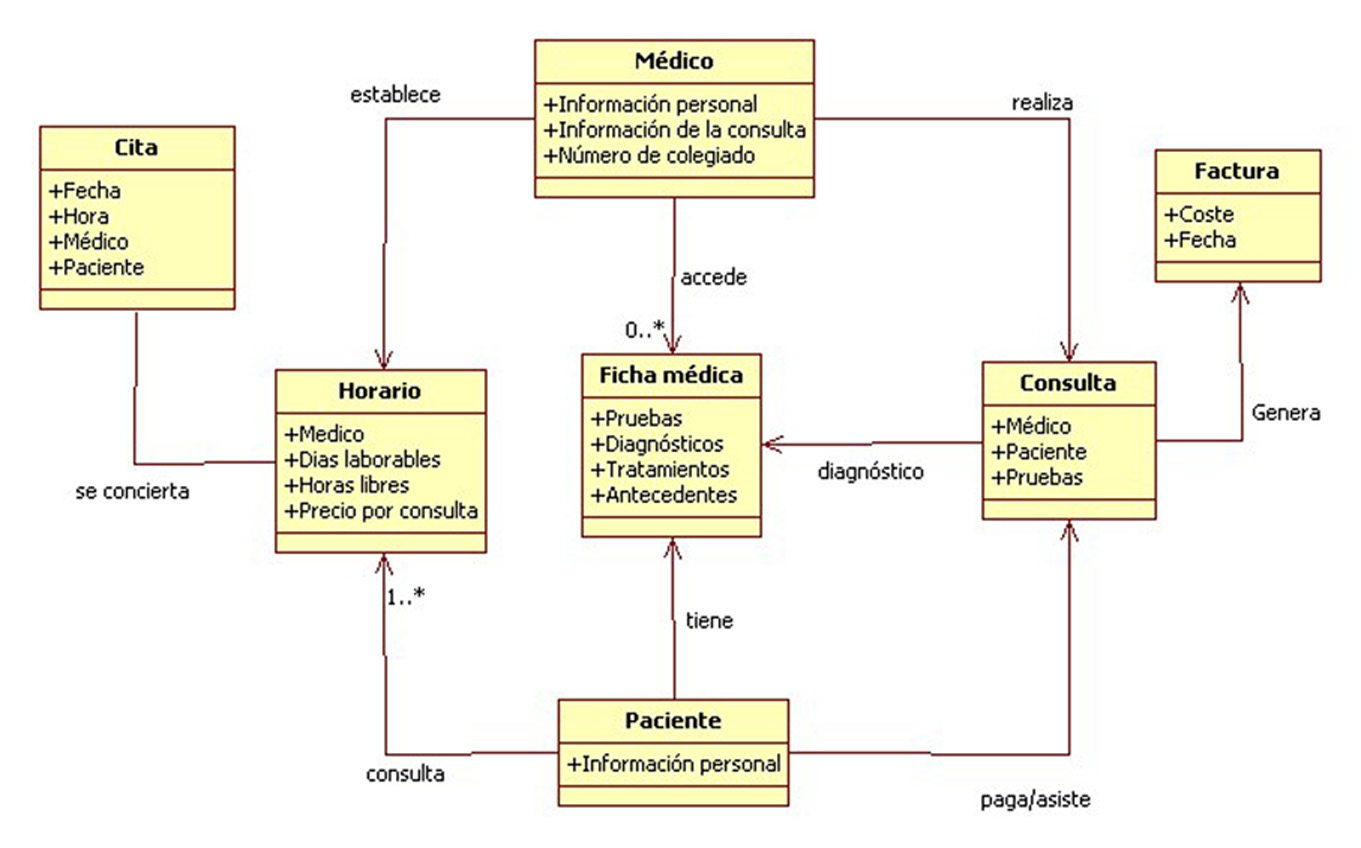
\includegraphics{img/modelo.jpg}
  \caption{Modelo del dominio}
  \label{modelodominio}
\end{figure}

\subsection{Glosario}
Acorde a lo visto en la Figura \ref{modelodominio} vamos a establecer un pequeño glosario.

\begin{itemize}
	\item \textbf{Cita.} Refleja que se concierta una consulta que supondrá el encuentro entre médico y paciente en la fecha y hora seleccionada. 
	\item \textbf{Consulta.} Encuentro entre médico y paciente.
	\item \textbf{Coste.} Transacción económica del importe de la consulta. 
	\item \textbf{Diagnóstico.} Calificación que da el médico a la enfermedad según los signos que advierte. Se añade a la ficha del paciente.
	\item \textbf{Factura.} Toda cita tiene un coste que debe ser abonado. Una vez realizado el pago, se genera una factura que corrobora que la transacción económica se ha producido.	
	\item \textbf{Ficha médica.} Información del paciente. Contiene tanto la información personal como todo tipo de información sanitaria: antecedentes, pruebas, diagnósticos, informes, tratamientos, etc.
	\item \textbf{Horario.} Horario del médico en el que aparece reflejado sus días laborables y sus horas disponibles, así como el coste de la consulta.
	\item \textbf{Médico.} Especialista encargado de la consulta con el paciente.
	\item \textbf{Paciente.} Persona con patología que acude a la consulta de un médico.
\end{itemize}


\end{document}